\documentclass[11pt, oneside]{article}   	% use "amsart" instead of "article" for AMSLaTeX format


%\usepackage{draftwatermark}
% \SetWatermarkText{Confidential}
% \SetWatermarkScale{5}
% \SetWatermarkLightness {0.85} 
% \SetWatermarkColor[rgb]{0.7,0,0}


\usepackage{geometry}                		% See geometry.pdf to learn the layout options. There are lots.
\geometry{letterpaper}                   		% ... or a4paper or a5paper or ... 
%\geometry{landscape}                		% Activate for for rotated page geometry
%\usepackage[parfill]{parskip}    		% Activate to begin paragraphs with an empty line rather than an indent
\usepackage{graphicx}				% Use pdf, png, jpg, or eps� with pdflatex; use eps in DVI mode
								% TeX will automatically convert eps --> pdf in pdflatex		
\usepackage{amssymb}
\usepackage{mathrsfs}
\usepackage{hyperref}
\usepackage{url}
\usepackage{subcaption}
\usepackage{authblk}
\usepackage{amsmath}
\usepackage{mathtools}
\usepackage{graphicx}
\usepackage{fixltx2e}
\usepackage{hyperref}
\usepackage{alltt}
\usepackage{color}
\usepackage[utf8]{inputenc}
\usepackage[english]{babel}

 
\newtheorem{theorem}{Theorem}[section]
\newtheorem{corollary}{Corollary}[theorem]
\newtheorem{lemma}[theorem]{Lemma}

\newcommand{\indep}{\raisebox{0.05em}{\rotatebox[origin=c]{90}{$\models$}}}
\newcommand{\argmax}{\operatornamewithlimits{argmax}}
\newcommand{\argmin}{\operatornamewithlimits{argmin}}
\DeclareMathOperator{\E}{\mathbb{E}}
\newcommand{\Var}{\mathrm{Var}}
\newcommand{\Cov}{\mathrm{Cov}}



\title{A Few Notes on Causal Inference}
\author{David Meyer \\ dmm@\{1-4-5.net,uoregon.edu\}}

\date{Last update: \today}							% Activate to display a given date or no date


\begin{document}
\maketitle

\section{Introduction}
Most studies in the sciences seek to answer causal rather than associative (i.e. statistical) questions. These questions require at least some knowledge of the data-generating process and cannot be computed from the data alone nor from the distributions that govern the data\footnote{This is a key result and was proven by Pearl  \cite{Pearl:2009:CMR:1642718}.} . Solving causal problems systematically requires certain extensions in the standard mathematical language of statistics, which include  (i) counterfactual analysis, (ii) nonparametric structural equations, (iii) graphical models, and (iv) the relationship between counterfactual and graphical methods. The bulk of this note will focus on these four areas.

\section{Association (statistics) vs. Causation}

The aim of standard statistical analysis is to assess parameters of a distribution from samples drawn of that distribution. Once we have an estimate of these parameters, we 
can infer statistical relationships (i.e. associations) among variables, which in turn allows us to estimate the probabilities of past and future events and update those 
probabilities in light of new information. In general, tasks of this sort are well treated by standard statistical analysis, so long as \emph{experimental conditions 
remain the same}. Causal analysis, on the other hand, goes one step further; its aim is to infer probabilities under conditions that are changing, for example, changes 
induced by treatments or external interventions.

\noindent
This distinction implies that causal and associational concepts do not mix; there is nothing in a joint distribution function that tells us how that distribution would change
if external conditions change, say from observational to experimental setup, because the laws of probability theory do not dictate how one property of a distribution ought
to change when another property is modified. This information must be provided by causal assumptions which identify relationships that remain invariant when external 
conditions change \cite{2015arXiv150101332P}.

\section{A Brief Introduction to Structural Equation Models}

How can one express mathematically the common understanding that symptoms do not cause diseases? The earliest attempt to formulate such relationship 
mathematically was made in the 1920's by the geneticist Sewall Wright \cite{wright1921}. Wright used a combination of equations and graphs to communicate 
causal relationships. For example, if $X$ stands for a disease variable and $Y$ stands for a certain symptom of the disease, Wright would write a linear equation\footnote{Linear equations are used here for illustration only; see e.g. \cite{2017arXiv170608576H} for examples using nonlinear models.} like
\begin{flalign}
Y = \beta X + U_y
\label{eqn:simple_linear}
\end{flalign}
where $X$ is the level or severity of a disease, $Y$ is the level (severity) of the symptom , and $u_y$ is a "noise" variable that represents all other than the disease in question
that could possibly affect $Y$ when $X$ is held constant. $Y$ is sometimes called the response variable and $X$ is frequently called the treatment. 

\begin{figure}
\center{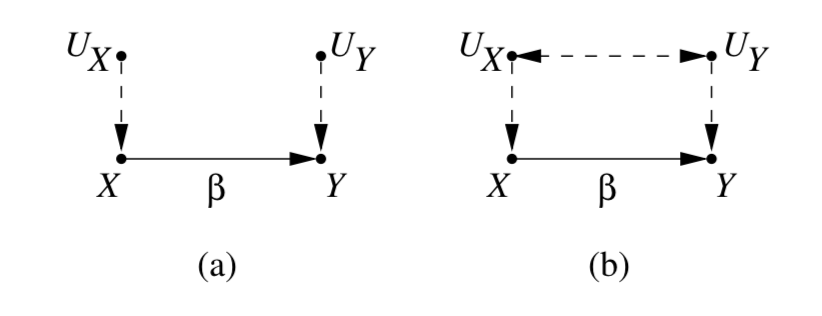
\includegraphics[scale=0.75] {images/simple_sem}}
\caption{A Simple Structural Equation Model (SEM), where $X = U_X$ and $Y = \beta X + U_Y$.  Unobserved exogenous variables are connected by dashed lines.}
\label{fig:simple_sem}
\end{figure}


\bigskip
\noindent
There is still a problem with Equation \ref{eqn:simple_linear} however, as it still does not properly express the causal relationship implied by this assignment process.
This is because algebraic equations are symmetrical objects; if we re-write Equation  \ref{eqn:simple_linear} as
\begin{flalign}
X = (Y - U_y)/\beta
\end{flalign}
could be misinterpreted to mean that the symptom influences the disease. To express the directionality of the underlying process, Wright augmented the equation with a diagram, 
later called "path diagram", in which arrows are drawn from (perceived) causes to their (perceived) effects, Importantly, the absence of an arrow makes the empirical 
claim that Nature assigns values to one variable irrespective of another.  For example, in Figure \ref{fig:simple_sem} the absence of arrow from $Y$ to $X$ represents 
the claim that symptom $Y$ is not among the factors $U_X$ which affect disease $X$. Thus, in our example, the complete model of a symptom and a disease would be 
written as in Figure \ref{fig:simple_sem}, where  the diagram encodes the possible existence of (direct) causal influence of $X$ on $Y$  and the absence of causal influence 
of $Y$ on $X$ , while the equations encode the quantitative relationships among the variables involved, to be determined from the data. The parameter $\beta$ in the 
equation is called a "path coefficient" and quantifies the direct causal effect of $X$ on $Y$, given $\beta$ and $U_Y$.  In particular,  the equation claims that, a unit increase 
in $X$ would result in $\beta$ units increase of $Y$ regardless of the values taken by other variables in the model\footnote{As we will see later, this property has many names, one of 
which is \emph{modularity.}}, regardless of whether the increase in $X$ originates from external or internal influences.

\bigskip
\noindent
The variables $U_X$ and $U_Y$ are called "exogenous",  as they represent observed or unobserved background factors that the modeler decides to keep unexplained, 
that is, factors that influence but are not influenced by the other variables (called "endogenous") in the model. Unobserved exogenous variables are sometimes called 
"disturbances" or "errors";  they represent factors omitted from the model but judged to be relevant for explaining the behavior of variables in the model. The variable $U_X$ , 
for example, represents factors that contribute to the disease $X$, which may or may not be correlated with $U_Y$, that is,  the factors that influence the symptom$Y$.

\bigskip
\noindent
In reading path diagrams, it is common to use kinship relations such as parent, child, ancestor, and descendent, the interpretation of which is usually self evident. 
For example, an arrow $X \rightarrow Y$ designates $X$ as a parent (cause) of $Y$ and $Y$ as a child of $X$. A "path" is any consecutive sequence of edges, solid 
or dashed. For example, there are two paths between $X$ and $Y$ in Figure  \ref{fig:simple_sem}(b):  one consisting of the direct arrow $X \rightarrow Y$ and the path
traces the nodes $X$, $U_X$, $U_Y$ and $Y$. We will see later that spurious associations such as Endogenous Selection Bias \cite{doi:10.1146/annurev-soc-071913-043455} 
can be transmitted on a path between two variables independent of the direction of the arrows on that path.

\bigskip
\noindent
Wright's major contribution to causal analysis, aside from introducing the language of path diagrams, has been the development of graphical rules for writing down 
the covariance of any pair of observed variables in terms of path coefficients and of covariances among the error terms. In the simple example in Figure \ref{fig:simple_sem}
we can immediately write down the covariance for Figure \ref{fig:simple_sem} (a) to be $\Cov(X,Y) = \beta$ and $\Cov(X,Y) = \beta + \Cov(U_X,U_Y)$ for 
Figure \ref{fig:simple_sem} (b). 

\bigskip
\noindent
Notice that in path diagrams, causal assumptions are encoded not in the links but, rather in the missing links. An arrow merely indicates the possibility of causal connection, 
the strength of which remains to be determined (from data); a missing arrow represents a claim of zero influence, while a missing double arrow represents a claim of 
zero covariance. For example, in Figure \ref{fig:simple_sem} (a), this assumptions that permits us to identify the direct effect $\beta$ are encoded by the missing
double arrow between $U_X$ and $U_Y$ and the missing arrow from $Y$ to $X$, indicating that $\Cov(U_Y,U_X)=0$. Had either or both of these two links been added 
to the diagram we would not have been able to identify the direct effect $\beta$ . Such additions would amount to relaxing the assumption $\Cov(U_Y , U_X ) = 0$ 
or the assumption that $Y$ does not effect $X$, respectively. Note also that both assumptions are causal, not associational, since neither can be determined from the 
joint density of the observed variables, $X$ and $Y$. In addition, the association between the unobserved terms, $U_Y$ and $U_X$ can only be uncovered in an 
experimental setting or by including additional  causal assumptions.

\begin{figure}
\center{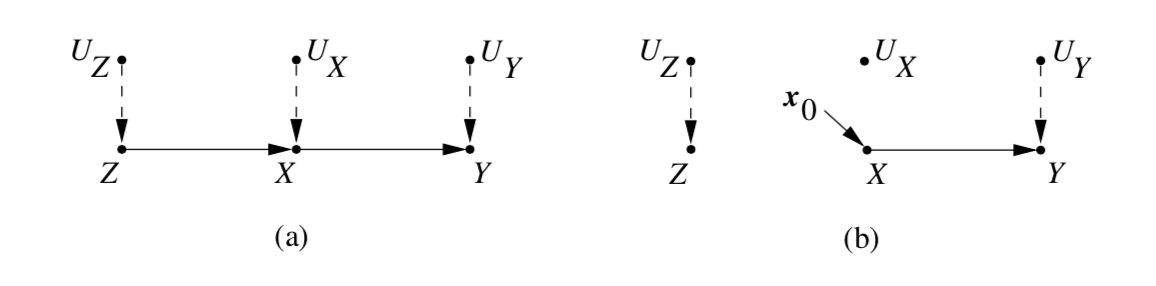
\includegraphics[scale=0.75] {images/chain_sem}}
\caption{A slightly more complex \emph{chain} SEM (a) and an intervention on $X$ (b)}
\label{fig:chain_sem}
\end{figure}

\bigskip
\noindent
Although each causal assumption in isolation cannot be tested, the sum total of all causal assumptions in a model often has testable implications. The chain model of 
Figure \ref{fig:chain_sem} (a), for example, encodes seven causal assumptions, each corresponding to a missing arrow or a missing double-arrow between a pair of 
variables. None of those assumptions is testable in isolation, yet the totality of all those assumptions implies that $Z$ is unassociated with $Y$ in every stratum of $X$ . 
Such testable implications can be read off the diagrams using a graphical criterion known as \emph{d-separation} \cite{Pearl:2009:CMR:1642718}. 

\bigskip
\noindent
\textbf{Definition 1} (d-separation) A set $S$ of nodes in a graph $G$ is said to \emph{block} a path $p$ if either (i) $p$ contains at least one arrow-emitting node that is in $S$, 
or (ii) $p$ contains at least one collision node (a "collider") that is outside $S$ and has no descendant in $S$. If $S$ blocks all paths from $X$ to $Y$,
$S$ is said to d-separate $X$ and $Y$. Moreover, if $X$ and $Y$ d-separated by $S$ then $X$ and $Y$ are (statistically) conditionally independent given $S$, 
written $X \indep Y | S$. That is

\begin{equation}
X \text{ and }  Y  \text{ d-separated by } S \implies X \indep Y | S
\end{equation}

\bigskip
\noindent
For example, in Figure \ref{fig:chain_sem} (a) the path $U_Z \rightarrow Z \rightarrow X \rightarrow Y$ is blocked by  $S = \{Z\}$ and by $S = \{X\}$
since each emits an arrow along that path. Consequently we can infer that the conditional independencies $U_Z \indep Y  |Z$ and $U_Z  \indep Y |X$ will be satisfied in 
any probability function that this model can generate, regardless of how we parametrize the arrows. Likewise, the path $U_Z \rightarrow Z \rightarrow X \leftarrow U_X$ is 
blocked by the null set $\{\emptyset\}$  but is not blocked by $S = \{Y\}$ since $Y$ is a descendant of the "collider"  $X$. It is an amazing result.

\bigskip
\noindent
As Pearl is fond of saying, d-separation is a "gift from the Gods" as it connects a property of a graph ($G$) with the joint distribution over $X$ and $Y$. That is, d-separation is
purely a property of graphs while conditional independence is a property of the (unknown) distributions of $X$, $Y$, and $S$.  $G$ will have to have certain properties, which we will 
have a look at in just a moment.
\newpage
\bibliographystyle{ieeetr}
\bibliography{/Users/dmm/papers/bib/ml}



\end{document} 
